\section{Dataset Construction}
We introduce the three-stage construction process of \ourdata: API collection (\cref{sec:api_collection}), instruction generation (\cref{sec:instruction_generation}), and solution path annotation (\cref{sec:answer_annotation}). All procedures are based on \turbo (\textit{gpt-3.5-turbo-16k}), requiring minimal human supervision and can be easily extended to new APIs. 

\subsection{API Collection}
\label{sec:api_collection}
We start by introducing RapidAPI and its hierarchy, followed by how we crawl and filter APIs.

\begin{figure*}[!t]
    \centering
    \subfigure{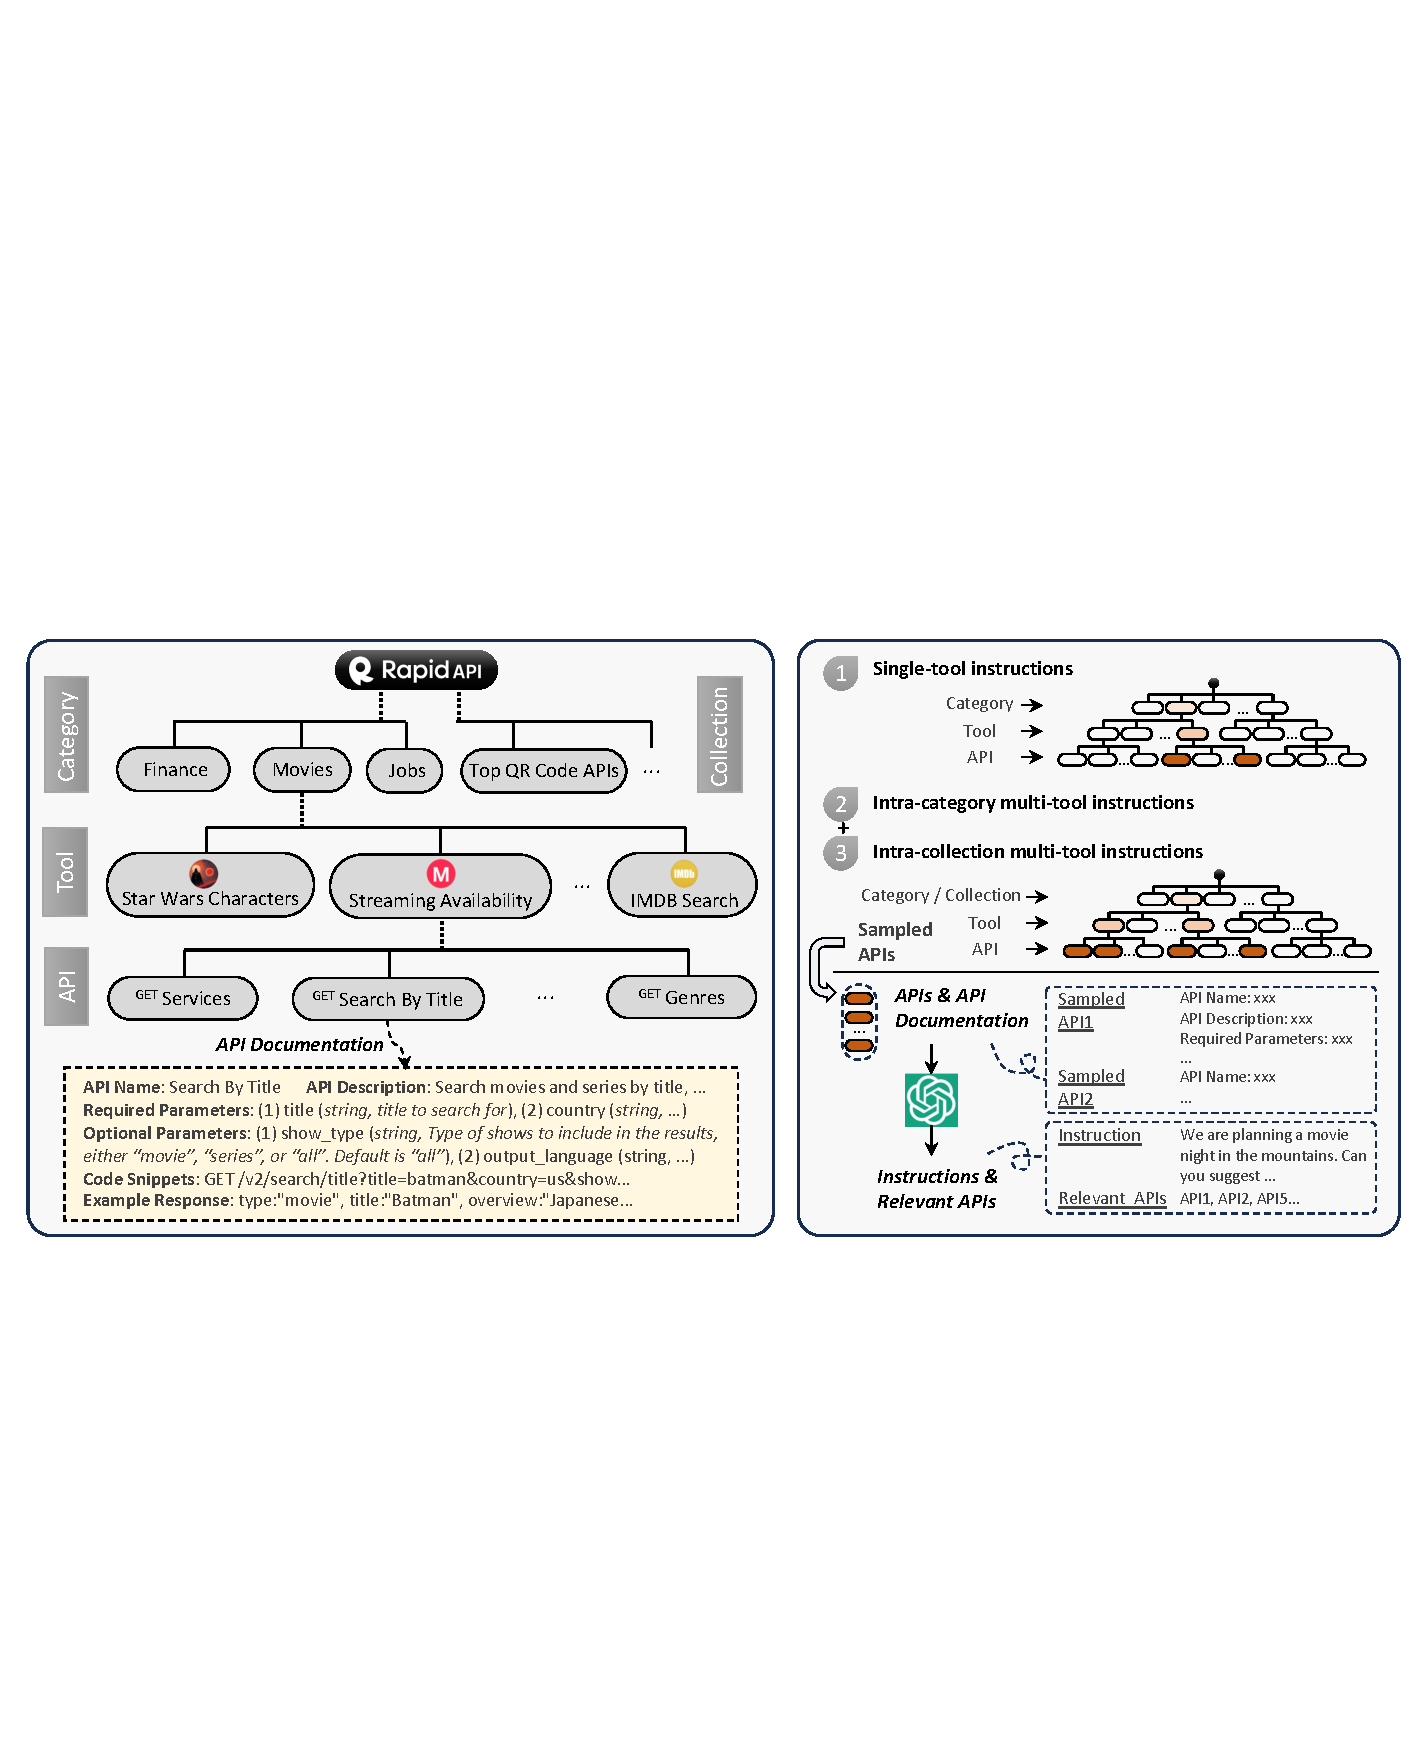
\includegraphics[width=\textwidth]{figs/phase12.pdf}}
    \caption{
    \small{The hierarchy of RapidAPI (left) and the process of instruction generation (right).}
    }
    \label{fig:phase12}
\end{figure*}

\textbf{RapidAPI Hub} \quad
RapidAPI is a leading API marketplace that connects developers with thousands of real-world APIs, streamlining the process of integrating diverse services into applications. Developers can test and connect with various APIs by registering only a RapidAPI key. All APIs in RapidAPI can be classified into $49$ \textit{coarse-grained} \textbf{categories} (\textcolor{blue}{\href{https://rapidapi.com/categories}{link}}), such as sports, finance, and weather. 
The categories associate an API with the most relevant topic.
Additionally, the hub also provides $500+$ \textit{fine-grained} categorization called \textbf{collections} (\textcolor{blue}{\href{https://rapidapi.com/collections}{link}}), e.g., Chinese APIs and database APIs. APIs in the same collection share a common characteristic and often have similar functionalities or goals.

\textbf{Hierarchy of RapidAPI} \quad
As shown in Figure~\ref{fig:phase12}, each tool may be composed of multiple APIs. For each tool, we crawl the following information: the name and description of the tool, the URL of the host, and all the available APIs belonging to the tool; for each API, we record its name, description, HTTP method, required parameters, optional parameters, request body, executable code snippets for API call, and an example API call response. This rich and detailed metadata serves as a valuable resource for LLMs to understand and effectively use the APIs, even in a zero-shot manner.

\textbf{API Filtering} \quad
Initially, we gathered $10,853$ tools ($53,190$ APIs) from RapidAPI. However, the quality and reliability of these APIs can vary significantly. In particular, some APIs may not be well-maintained, such as returning 404 errors or other internal errors.
To this end, we perform a rigorous filtering process (details in \cref{sec:detail_filtering_api}) to ensure that the ultimate tool set of \ourdata is reliable and functional.
Finally, we only retain $3,451$ high-quality tools ($16,464$ APIs).

\subsection{Instruction Generation}
\label{sec:instruction_generation}

Different from prior works, we specifically focus on two crucial aspects for instruction generation: (1) \textbf{diversity}: to train LLMs to handle a wide range of API usage scenarios, thereby boosting their generalizability and robustness; and (2) \textbf{multi-tool usage}: to mirror real-world situations that often demand the interplay of multiple tools, improving the practical applicability and flexibility of LLMs. 
To this end, instead of brainstorming instructions from scratch and then searching for relevant APIs, we sample different combinations of APIs and craft various instructions that involve them.
% In practice, this strategy ensures the coverage for all collected APIs.
% Furthermore, we use the RapidAPI hierarchy to identify tool relationships, which aids in the generation of multi-tool instructions.

\textbf{Generating Instructions for APIs} \quad
Define the total API set as $\sS_\text{API}$, at each time, we sample a few APIs: $\sS_\text{N}^{\text{sub}} \!=\! \{\text{API}_1, \cdots, \text{API}_\text{N}\}$ from $\sS_\text{API}$. We prompt \turbo to understand the functionalities of these APIs and then generate (1) possible instructions ($\text{Inst}_*$) that involve APIs in $\sS_\text{N}^{\text{sub}}$, and (2) relevant APIs ($\sS_*^{\text{rel}} \!\subset\!\sS_\text{N}^{\text{sub}}$) for each instruction ($\text{Inst}_*$), i.e., $\{[\sS_1^{\text{rel}}, \text{Inst}_1], \cdots, [\sS_{\text{N}'}^{\text{rel}}, \text{Inst}_{\text{N}'}]\}$, where $\text{N}'$ denotes the number of generated instances.
These (instruction, relevant API) pairs will be used for training the API retriever in \cref{sec:prelim_exp}.
We use different sampling strategies (introduced later) to cover all APIs and most of their combinations, thus ensuring the diversity of our instructions.

The prompt for \turbo is composed of (1) a general description of the intended instruction generation task, (2) comprehensive documentation of each API in $\sS_\text{N}^{\text{sub}}$, which helps \turbo understand their functionality and interplay, and (3) three in-context seed examples $\{\text{seed}_1, \text{seed}_2, \text{seed}_3\}$. Each seed example is an ideal instruction generation written by human experts. These seed examples are leveraged to better regulate \turbo's behavior through in-context learning. In total, we wrote $12$ / $36$ diverse seed examples ($\sS_\text{seed}$) for the single-tool / multi-tool setting, and randomly sampled three examples at each time. Detailed prompts for instruction generation are described in \cref{sec:inst_prompt}. Overall, the generation process can be formulated as follows:
\begin{equation}
    \small
    \begin{aligned}
    \underset{\{\text{API}_1, \cdots, \text{API}_\text{N}\} \in \sS_{\text{API}}, \{\text{seed}_1, \cdots, \text{seed}_3\} \in \sS_\text{seed}}{\text{\turbo}}(\{[\sS_1^{\text{rel}}, \text{Inst}_1], \cdots, [\sS_{\text{N'}}^{\text{rel}}, \text{Inst}_{\text{N}'}]\} | \text{API}_1, \cdots, \text{API}_\text{N}, \text{seed}_1, \cdots, \text{seed}_3).
        \nonumber
    \end{aligned}
    \label{eq:instruction_generation}
\end{equation}

% \underset{\substack{\{\text{API}_1, \cdots, \text{API}_\text{N}\} \in \sS_{\text{API}}, \\ \{\text{seed}_1, \cdots, \text{seed}_3\} \in \sS_\text{seed}}}{\text{\turbo}}(\{[\sS_1^{\text{rel}}, \text{Inst}_1], \cdots, [\sS_{\text{N'}}^{\text{rel}}, \text{Inst}_{\text{N}'}]\} | \text{API}_1, \cdots, \text{API}_\text{N}, \text{seed}_1, \cdots, \text{seed}_3).


\textbf{Sampling Strategies for Different Scenarios} \quad
As shown in Figure~\ref{fig:phase12}, for the \textbf{single-tool instructions (I1)}, we iterate over each tool and generate instructions for its APIs. However, for the \textbf{multi-tool setting}, since the interconnections among different tools in RapidAPI are sparse, random sampling tool combinations from the whole tool set often leads to a series of irrelevant tools that cannot be covered by a single instruction in a natural way. To address the sparsity issue, we leverage the RapidAPI hierarchy information.
Since tools belonging to the same RapidAPI \textit{category} or \textit{collection} are generally related to each other in the functionality and goals, we randomly select $2$-$5$ tools from the same category / collection and sample at most $3$ APIs from each tool to generate the instructions. We denote the generated instructions as \textbf{intra-category multi-tool instructions (I2)} and \textbf{intra-collection multi-tool instructions (I3)}, respectively. Through rigorous human evaluation, we find that instructions generated in this way already have a high diversity that covers various practical scenarios. We also provide visualization for instructions using Atlas (\textcolor{blue}{\href{https://atlas.nomic.ai/map/58aca169-c29a-447a-8f01-0d418fc4d341/030ddad7-5305-461c-ba86-27e1ca79d899}{link}}) to support our claim.

\begin{figure*}[!t]
    \centering
    \subfigure{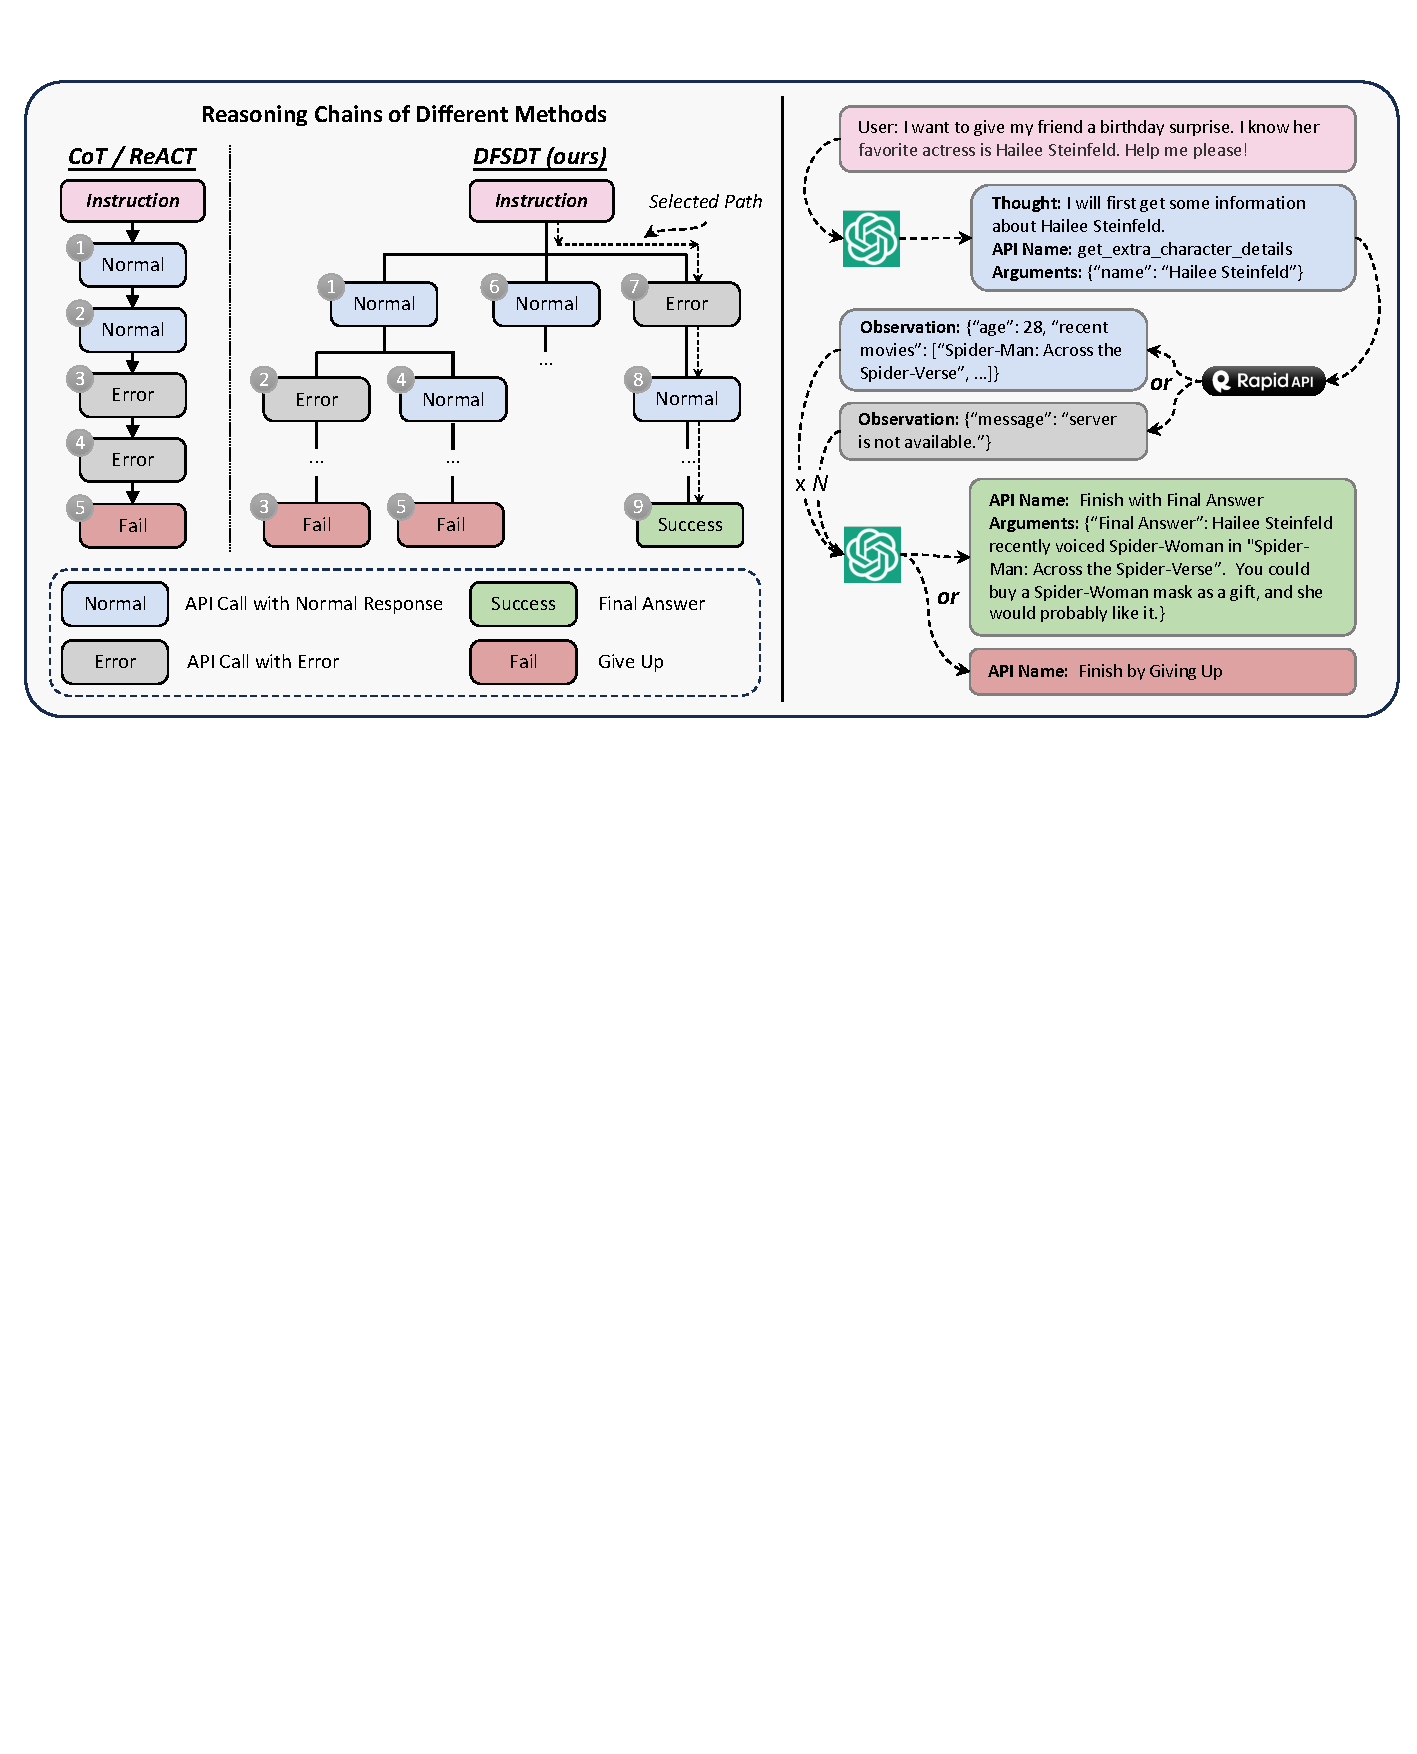
\includegraphics[width=\textwidth]{figs/answer_anno.pdf}}
    \caption{
    \small{A comparison of our \dfs and conventional CoT or ReACT during model reasoning (left). We show part of the solution path annotation process using \turbo (right).}
    }
    \label{fig:phase3}
\end{figure*}

After generating the initial set of instructions, we further filter those with the hallucinated relevant APIs by assessing whether they exist in $\sS_\text{N}^{\text{sub}}$.
Finally, we collect nearly $200$k qualified (instruction, relevant API) pairs, including $87413$, $84815$, and $25251$ instances for I1, I2, and I3, respectively.

\subsection{Solution Path Annotation}
\label{sec:answer_annotation}
As shown in Figure~\ref{fig:phase3}, given an instruction $\text{Inst}_*$, we prompt \turbo to search for a valid action sequence: $\{a_1, \cdots, a_\text{N}\}$. Such a multi-step decision-making process is cast as a multi-round conversation for \turbo. At each round $t$, the model generates an action $a_t$ based on previous interactions, i.e., $\text{\turbo}(a_t|\{a_1, r_1, \cdots, a_{t-1}, r_{t-1}\}, \text{Inst}_*)$, where $r_*$ denotes the real API response.
For each $a_t$, \turbo should specify its ``thought'',  which API to use, and the specific parameters for this API, i.e., $a_t$ has the following format: ``\texttt{Thought}: $\cdots$, \texttt{API Name}: $\cdots$, \texttt{Parameters}: $\cdots$''.
% Hence the decision space is the Cartesian product of the thought, available APIs, and possible parameters, which is infinite by nature.

To leverage the \textbf{function call} feature of \turbo, we treat each API as a special function and feed its API documentation into \turbo's function field. In this way, the model understands how to call the API. For each instruction $\text{Inst}_*$, we feed all the sampled APIs $\sS_\text{N}^{\text{sub}}$ to \turbo's as available functions.
To let \turbo finish an action sequence, we define two additional functions, i.e., ``Finish with Final Answer'' and ``Finish by Giving Up''. The former function has a parameter that corresponds to a detailed final answer to the original instruction; while the latter function is designed for cases where the provided APIs cannot complete the original instruction after multiple API call attempts.
% instead of only its relevant APIs $\sS_*^{\text{rel}}$. In this way, the model gains access to a broader scope of APIs and expands the action space.

\textbf{Depth First Search-based Decision Tree} \quad
In our pilot studies, we find that CoT~\citep{wei2023chainofthought} or ReACT~\citep{yao2022react} has inherent limitations: (1) \textbf{error propagation}: a mistaken action may propagate the errors further and cause the model to be trapped in a faulty loop, such as continually calling an API in a wrong way or hallucinating APIs; (2) \textbf{limited exploration}: CoT or ReACT only explores one possible direction, leading to limited exploration of the whole action space. Hence even GPT-4 often fails to find a valid solution path, making annotation difficult.

To this end, we propose to construct a decision tree to expand the search space and increase the possibility of finding a valid path. As depicted in Figure~\ref{fig:phase3}, our \dfs allows the model to assess different reasoning paths and choose to either (1) proceed along a promising path or (2) abandon an existing node by calling the ``Finish by Giving Up'' function and expand a new node. During node expansion, to diversify the child nodes and expand the search space, we prompt \turbo with the information of the previously generated nodes and explicitly encourage the model to generate a distinct node. For the searching process, we prefer depth-first search (DFS) instead of breadth-first search (BFS) because the annotation can be finished as long as one valid path is found. Using BFS will cost excessive OpenAI API calls. More details are described in \cref{sec:answer_prompt}.
% before reaching a terminal node (the node of ``Finish with Final Answer'' or ``Finish by Giving Up'').
We perform \dfs for all the generated instructions and only retain those passed solution paths. Ultimately, we generate $126,486$ (instruction, solution path) pairs, which are used to train \ourmodel in \cref{sec:main_exp}. % Although it is possible to construct more training instances, we find that $12,657$ instances already bring satisfying generalization performance.